\documentclass[preprintnumbers,amsmath,amssymb,onecolumn,12pt]{revtex4}
\usepackage{graphicx}% Include figure files
\usepackage{dcolumn}% Align table columns on decimal point
\usepackage{bm}% bold math
\usepackage{natbib}
\usepackage{physics}
\usepackage[caption=false]{subfig}
\newcommand{\be}{\begin{equation}}
\newcommand{\ee}{\end{equation}}

\newcommand{\bea}{\begin{eqnarray}}
\newcommand{\eea}{\end{eqnarray}}
 
\def\sgn{\mathop{\rm sgn}}

\begin{document}

\vspace{0.2in}
{\Large \hspace{1.6in}\textsc{Supplementary Material} }\\
\
\title{Observation of a Magnetic-Torque Enhanced by Interacting Spin Ensembles}

\author{C. Pellet-Mary$^1$, P. Huillery$^1$, M. Perdriat$^1$, G. H\'etet$^1$} 


\affiliation{$^1$
Laboratoire de Physique de l'Ecole normale sup\'erieure, ENS, Universit\'e PSL, CNRS, Sorbonne Universit\'e, Universit\'e Paris-Diderot, Sorbonne Paris Cit\'e, Paris, France.
}


\maketitle

\tableofcontents


\section{NV$^-$ center Theory}
\subsection{NV spin hamiltonian}
The hamiltonian of the electronic spin of the negatively charged nitrogen-vacancy center in its ground state can be written as :
\begin{equation*}
  \hat{\mathcal{H}}_s=\hbar D S_{z'}^2 + \hbar \gamma_e \textbf{B}\cdot\hat{\textbf{S}},
  \end{equation*} 
where $D = (2\pi) 2.87$ GHz is the crystal field splitting originating from spin-spin interactions, and $\gamma_e = 28 $GHz/T is the electron gyromagnetic ratio. 
The \textbf{z'} axis in the $S_{z'}$ operator here is the axis formed by the nitrogen atom and the vacancy in the body fixed frame.
We neglect contributions from the strain and local electric field in the hamiltonian since we are working with magnetic fields on the order of 10 mT, which induce splittings larger than the splitting of the zero-field ESR line ($\approx 20$ MHz). We also neglect the hyperfine interaction with the nuclear spin of the $^{14}$N atom since we are working with ensembles with typical inhomogeneous broadening of 5~MHz. 

% hence why we do have different energy transitions for different NV orientations, depending on the projection of the magnetic field on the NV axis.

\subsection{Diamond crystalline axes and degeneracy conditions}
\begin{figure}[!ht]
  \centering \scalebox{0.45}{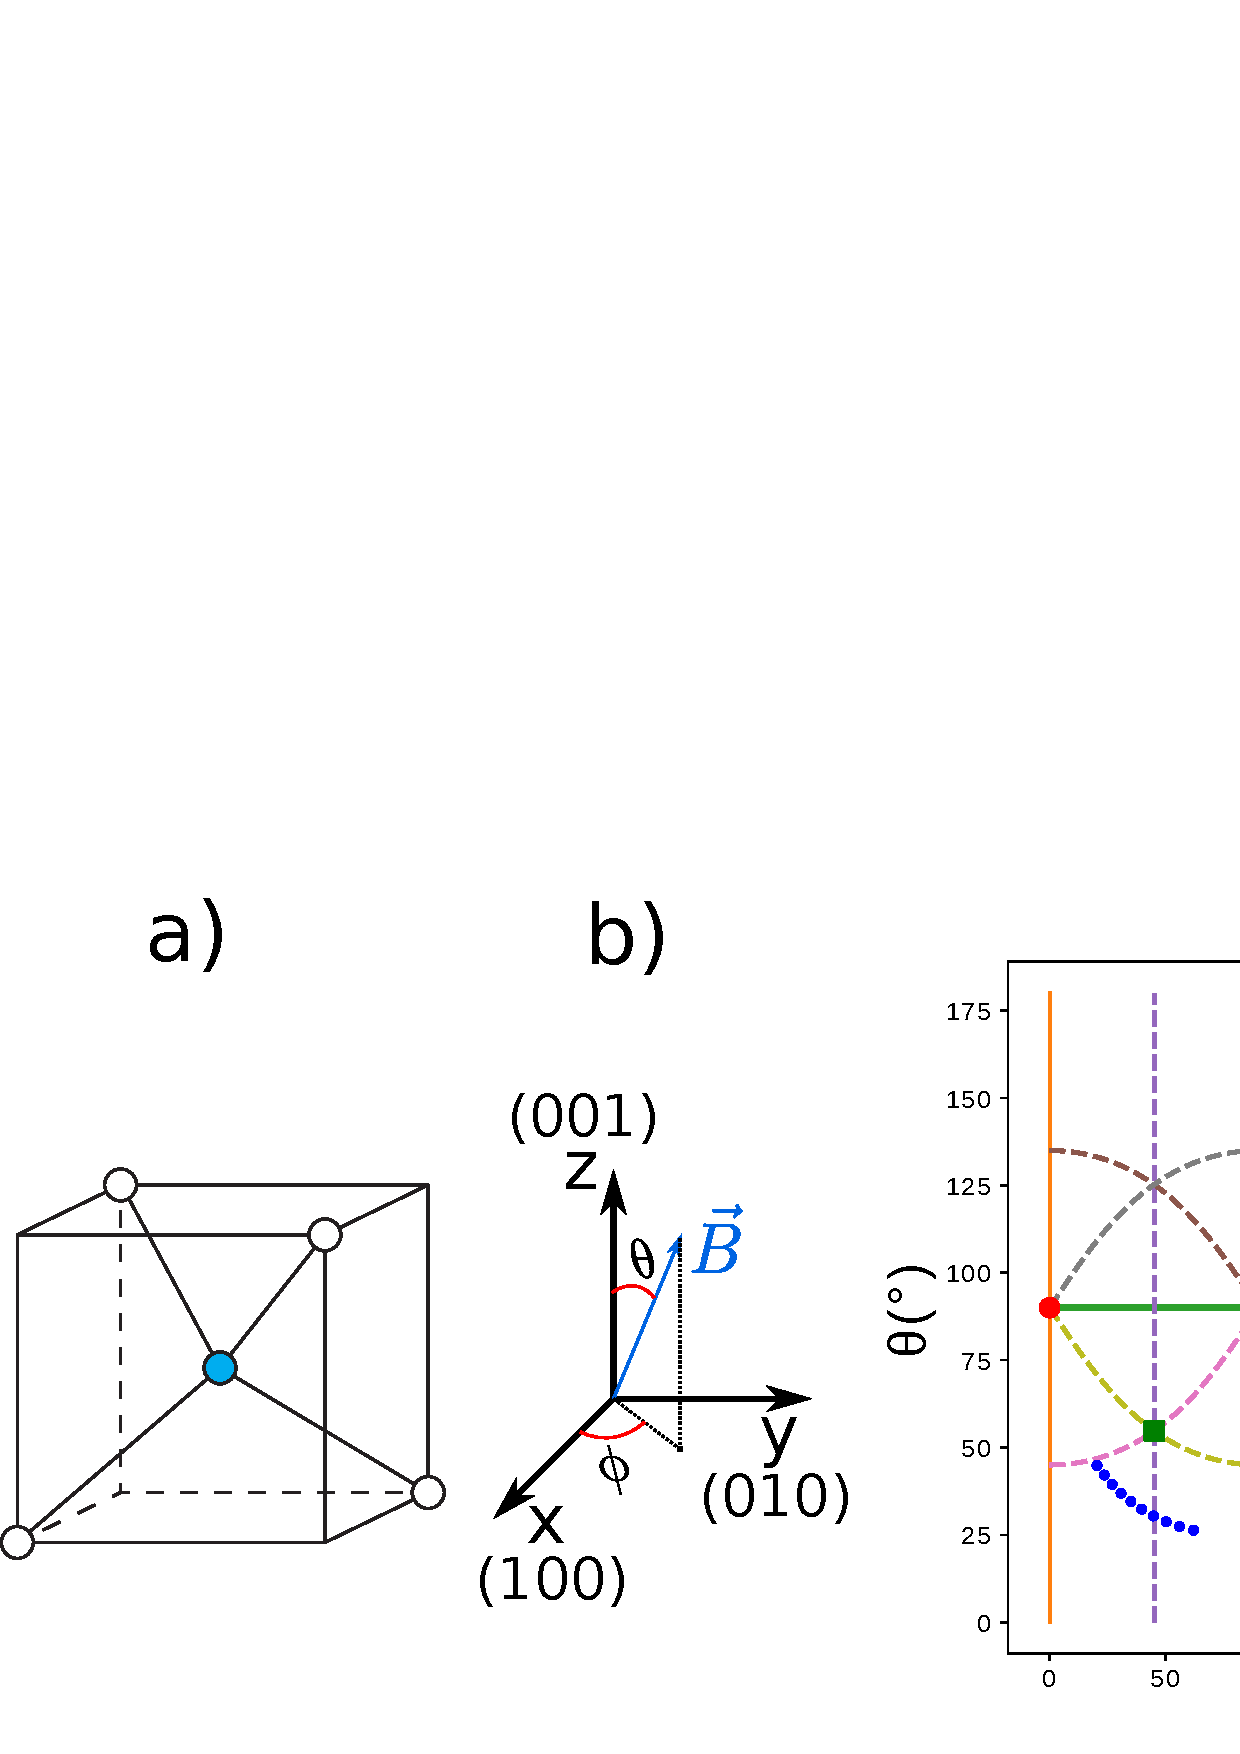
\includegraphics{SI_Cristallo}}
  \caption{a) Representation of the four crystalline axes of the diamond b) Representation of the magnetic field in the diamond crystalline basis c) Representation of the crystalline planes in the $(\theta , \phi)$ basis. The $\{ 110 \}$ family of planes are shown using dashed lines and the $\{ 110 \}$ family using plain lines. The [100] direction is marked by red circles, the [111] direction by green squares. The magnetic field path in the experiment of Fig. 3 of the main text is shown with blue dots.}
	\label{cristallo}
\end{figure}
There are four possible crystalline axes for the N-V direction (so-called ``classes" of NV) in the diamond. They are depicted in Fig. \ref{cristallo} b) and correspond to the crystalline directions [$111$], [$1\bar 1 \bar 1$], [$\bar 1 1 \bar 1$] and [$\bar 1 \bar 1 1$]. 

The magnetic field direction is represented in Fig. \ref{cristallo} a), where the usual polar and azimuthal angles $\theta$ and $\phi$ are defined with respect to the \textbf{z'} ([$001$]) direction (we denote with ' the axes in the diamond frame). For some orientations of the magnetic field, the projection of the magnetic field on two or more NV axes will be identical, and therefore the energy level of the corresponding classes will be the same. These degeneracies are represented in Fig \ref{cristallo} c), where the dashed lines are the locii of the $\{ 110 \}$ family of planes (plane normal to the [110] direction and all other equivalent directions, making 6 planes in total). When the magnetic field belongs to these planes, we observe a degeneracy between two classes of NVs, as can be seen in the Fig.\ref{scan_dege} or in Fig. 4 of the main paper.

The plain lines are the locii of the $\{ 100 \}$ family of planes (3 planes in total). When the magnetic field lies in these planes, all classes are co-resonant, as can be seen in Fig.\ref{scan_dege} or in Fig.\ref{CR_22}.
The red circles correspond to the [100] directions, for which the four classes of NV are degenerate. The green squares correspond to the [111] direction where one class is aligned with the magnetic field, and the three others are degenerate. Finally the blue dots correspond to the path followed by the magnetic field in the experiment presented in Fig 3 of the main text, where we can see that a plane from the $\{ 110 \}$ family is being crossed.

\section{Depolarization induced by NV-NV cross-relaxation}
As explained in the main text, when the density of NV$^-$ centers in the sample is high enough (typically for concentrations higher than 1 ppm), the ensemble of NV spins will lose some of its polarization through dipolar coupling between the NV centers. This phenomenon is at the heart of the mechanism that allows us to exalt the magnetic suceptibility of our diamond through dipolar interaction, and it has already been observed independently by many groups in bulk diamond \cite{Jarmola} \cite{mrozek_longitudinal_2015} \cite{choi_depolarization_2017} \cite{akhmedzhanov_microwave-free_2017} \cite{giri_coupled_2018}

In particular, \cite{choi_depolarization_2017} proposes a model based on "fluctuators" : a subgroup of NV centers with a very short lifetime (possibly due to their electron tunnelling in and out of the NV site) that can act as a source of classical noise with a central frequency given by the usual transition frequencies of the NV$^-$ spin Hamiltonian. A prediction of this model is that the modified lifetime of the ensemble of NV centers should have a stretch exponential profile (of the form $e^{-\sqrt{\frac{t}{T_1}}}$) which we do observe experimentally.

\subsection{Stretch exponential profile of the lifetimes}
\begin{figure}
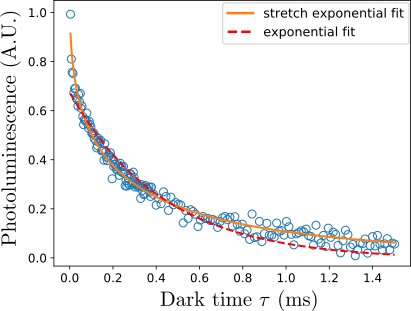
\includegraphics[scale=0.7]{T1-stretch_exp}
\caption{Lifetime measurement for a case where all four classes are degenerate. Plain orange line correspond to a stretch-exponential fit and dashed red line to a simple exponential fit}
	\label{stretch}
\end{figure}
In the theory developed in \cite{choi_depolarization_2017}, the stretch exponential profile arises from the inhomogeneity of the distance from each NV centers to the closest fluctuators. If $\rho_{00}^s(t)$, the population in the $\ket{m_s=0}$ state for each NV centers evolving in the dark, follow a law of the form $\rho_{00}^s(t) \propto \exp(-\gamma t)$ where $\gamma$ is the individual depolarization rate of the spin; then, assuming an even spatial distribution of fluctuators, the authors of \cite{choi_depolarization_2017} show that the distribution in $\gamma$ should follow a law of the form $$\rho(\gamma) \approx \frac{e^{-\frac{1}{4 \gamma T_1}}}{\sqrt{4 \pi \gamma^3 T_1}} $$ where $\rho(\gamma)$ is the density of probability of $\gamma$.

Averaging then over all NV centers gives the stretch exponential profile observed from the ensemble :
$$ \rho_{00}^e(t) \propto \int_0^{+\infty} \rho(\gamma) e^{-\gamma t} d\gamma = e^{-\sqrt{\frac{t}{T_1}}} $$
where $ \rho_{00}^e(t)$ correspond to the average population in the $\ket{m_s=0}$ state for the ensemble of spins.

Fig. \ref{stretch} shows a lifetime measurement on a static micro diamond following the protocol described in Sec.III. Here all four classes are resonant with the applied microwave frequency, which corresponds to the maximum degree of degeneracy between the NV centers, and therefore the stronger modification of the lifetime induced by the resonant dipolar coupling. The signal we obtain was fitted using a stretch exponential profile  and a simple exponential profile. We can see that the stretch exponential profile ($R^2=0.981$) is in better agreement with the data than the exponential fit ($R^2=0.942$), in particular for the very short times (we expect the longer times to be dominated by the phonon-limited exponential lifetime).

Finally it should be noted that the stretch exponential profile arising from point-like depolarization sources is a relatively general result that has for example also been observed for the depolarization of NV centers induced by substitutional nitrogen (P1) defects in diamond \cite{hall_detection_2016}

\subsection{Scanning the degeneracy conditions}
\begin{figure}
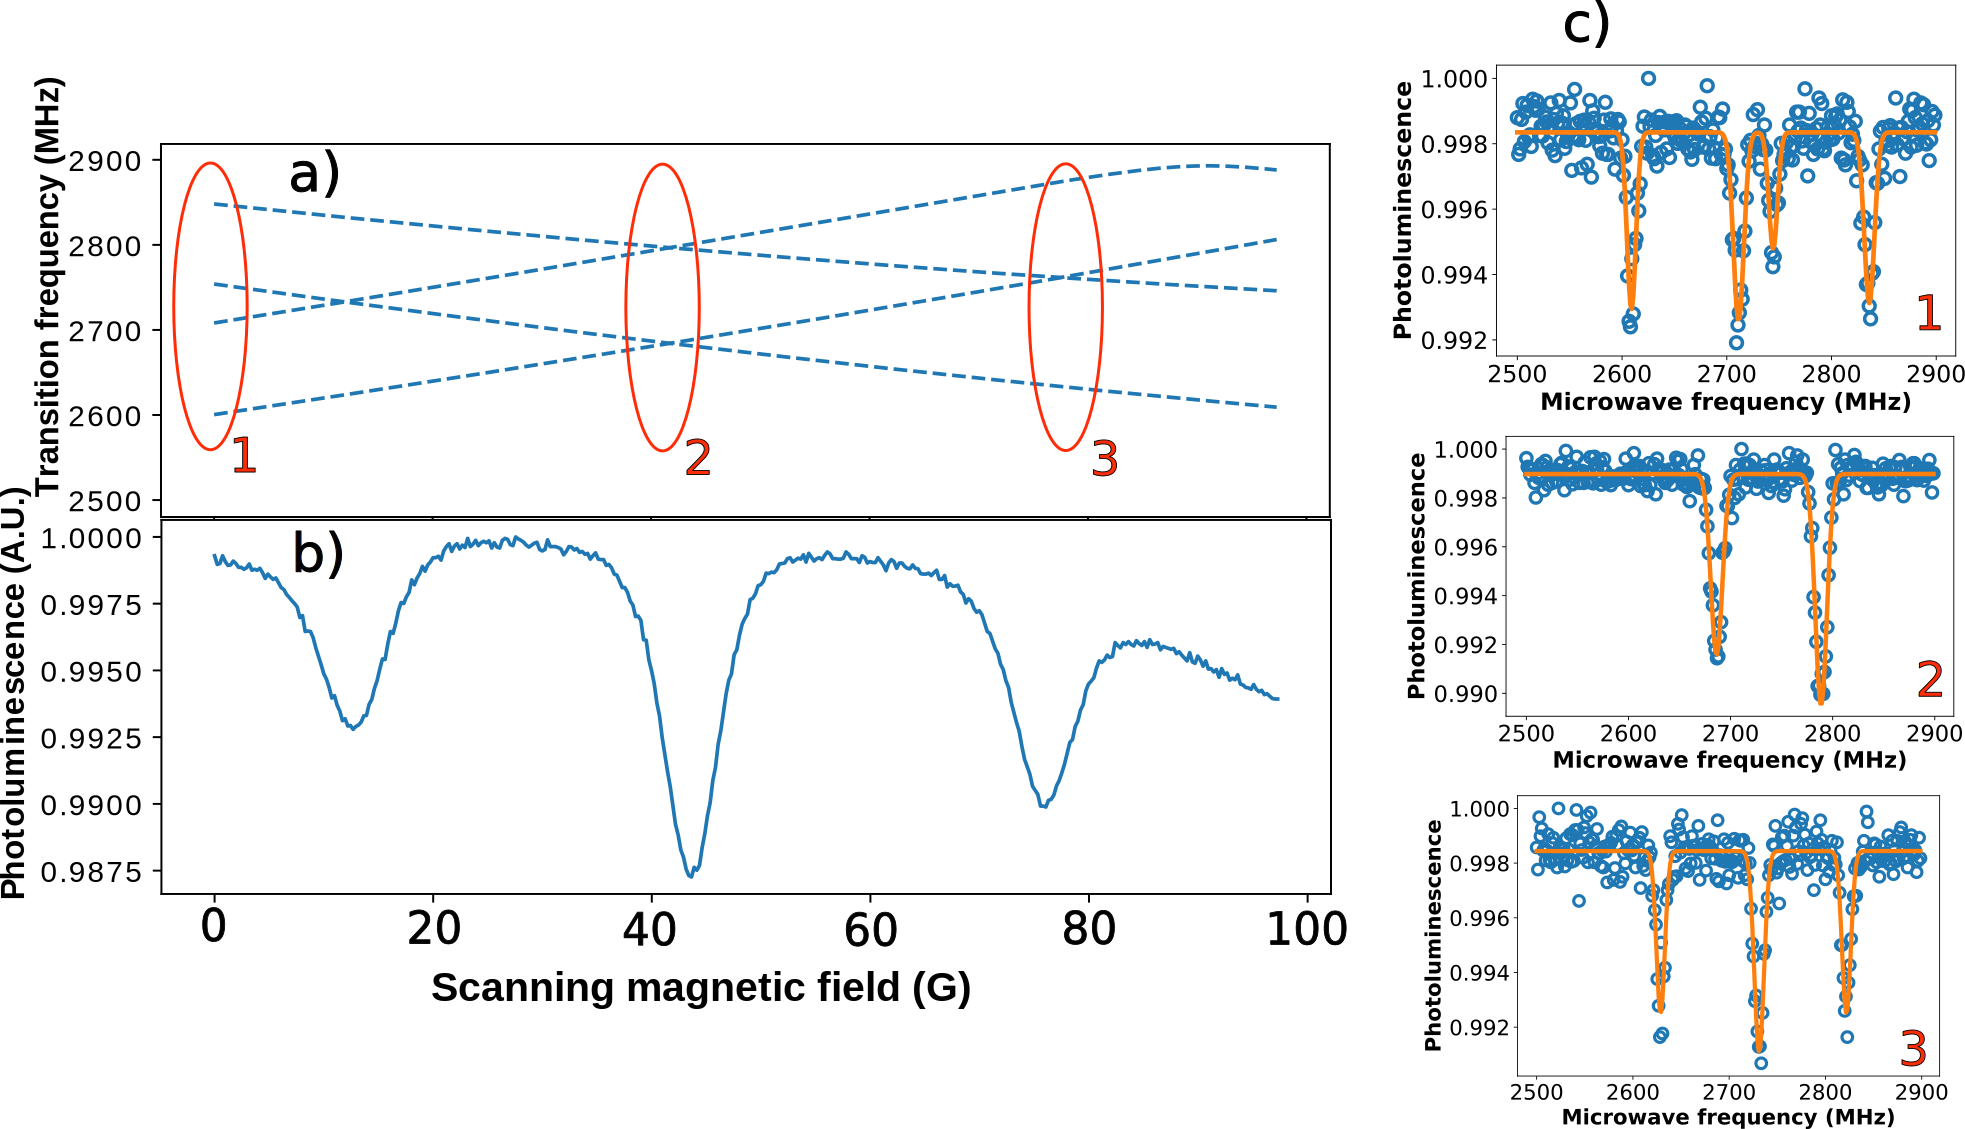
\includegraphics[scale=0.3]{scan_CR}
\caption{Experimental results for a magnetic field scan with an electromagnet while a static magnetic field offset is applied with a permanent magnet (setup similar to the one presented in Fig.\ref{Optics}) \textbf{a)} Frequency Transitions for the $\ket{m_s=0} \to \ket{m_s=-1}$ transition of the four classes of NV centers as a function of the scanning magnetic field (data extrapolated from ODMR spectra) \textbf{b)} Change in photoluminescence of the NV$^-$ centers as a function of the scanning magnetic field. \textbf{c)} Example of 3 ODMR spectra for the 3 particular field values corresponding to the circled areas in subfigure a).}
	\label{scan_dege}
\end{figure}
The easiest way to probe the mechanism of dipolar-induced modification of the lifetime is to change the degeneracy conditions between the four classes of NV centers by tuning the magnetic field, as explained in Sec.I.
Because the NV spins can only exchange spin quanta when they are quasi-resonant, then by tuning the number of classes at degeneracy, you can modify the effective density of interacting NV centers, and therefore tune the depolarization effect. 

An example of this is given in Fig.2 of the main text with the varying lifetime depending on the degeneracy condition, but another way to probe this effect is shown in Fig.\ref{scan_dege} : in this figure, we have observed the change in photoluminescence from a static microdiamond while changing the magnetic field in order to explore different degeneracy conditions. In order to do this, we need two sources of magnetic field : an electromagnet to scan the field and a permanent magnet to apply a magnetic field offset in an other direction (otherwise the magnetic field orientation with respect to the diamond axes would remain the same as the field is scanned).

In this particular case, we can see that as the magnetic field is scanned, it crosses three "degeneracy planes" (as described in Sec.I) : first a plane of the the $\{ 110 \}$ family at B=13 G, with a single degeneracy condition, then a plane of the $\{ 100 \}$ family at B=44 G where there is a simultaneous degeneracy condition for two pairs of classes, and then another plane of the the $\{ 110 \}$ family at B=76 G. We notice that each time a degeneracy between at least two classes of NV happens, we observe in Fig.\ref{scan_dege}b) a sharp decrease in photoluminescence. This is a signature of the change in lifetime of the ensemble of spins : indeed, the photoluminescence of NV ensembles is proportional to the average population in the $\ket{m_s=0}$ state, and the $\ket{m_s=0}$ population of the spins is the result of the competition between the polarization rate due to the green laser and the various depolarization mechanism. Increasing the depolarization rate of the spins will therefore decrease the overall luminosity.



\section{Experimental details}

\subsection{Experimental setup}

\begin{figure}[!ht]
  \centering \scalebox{0.3}{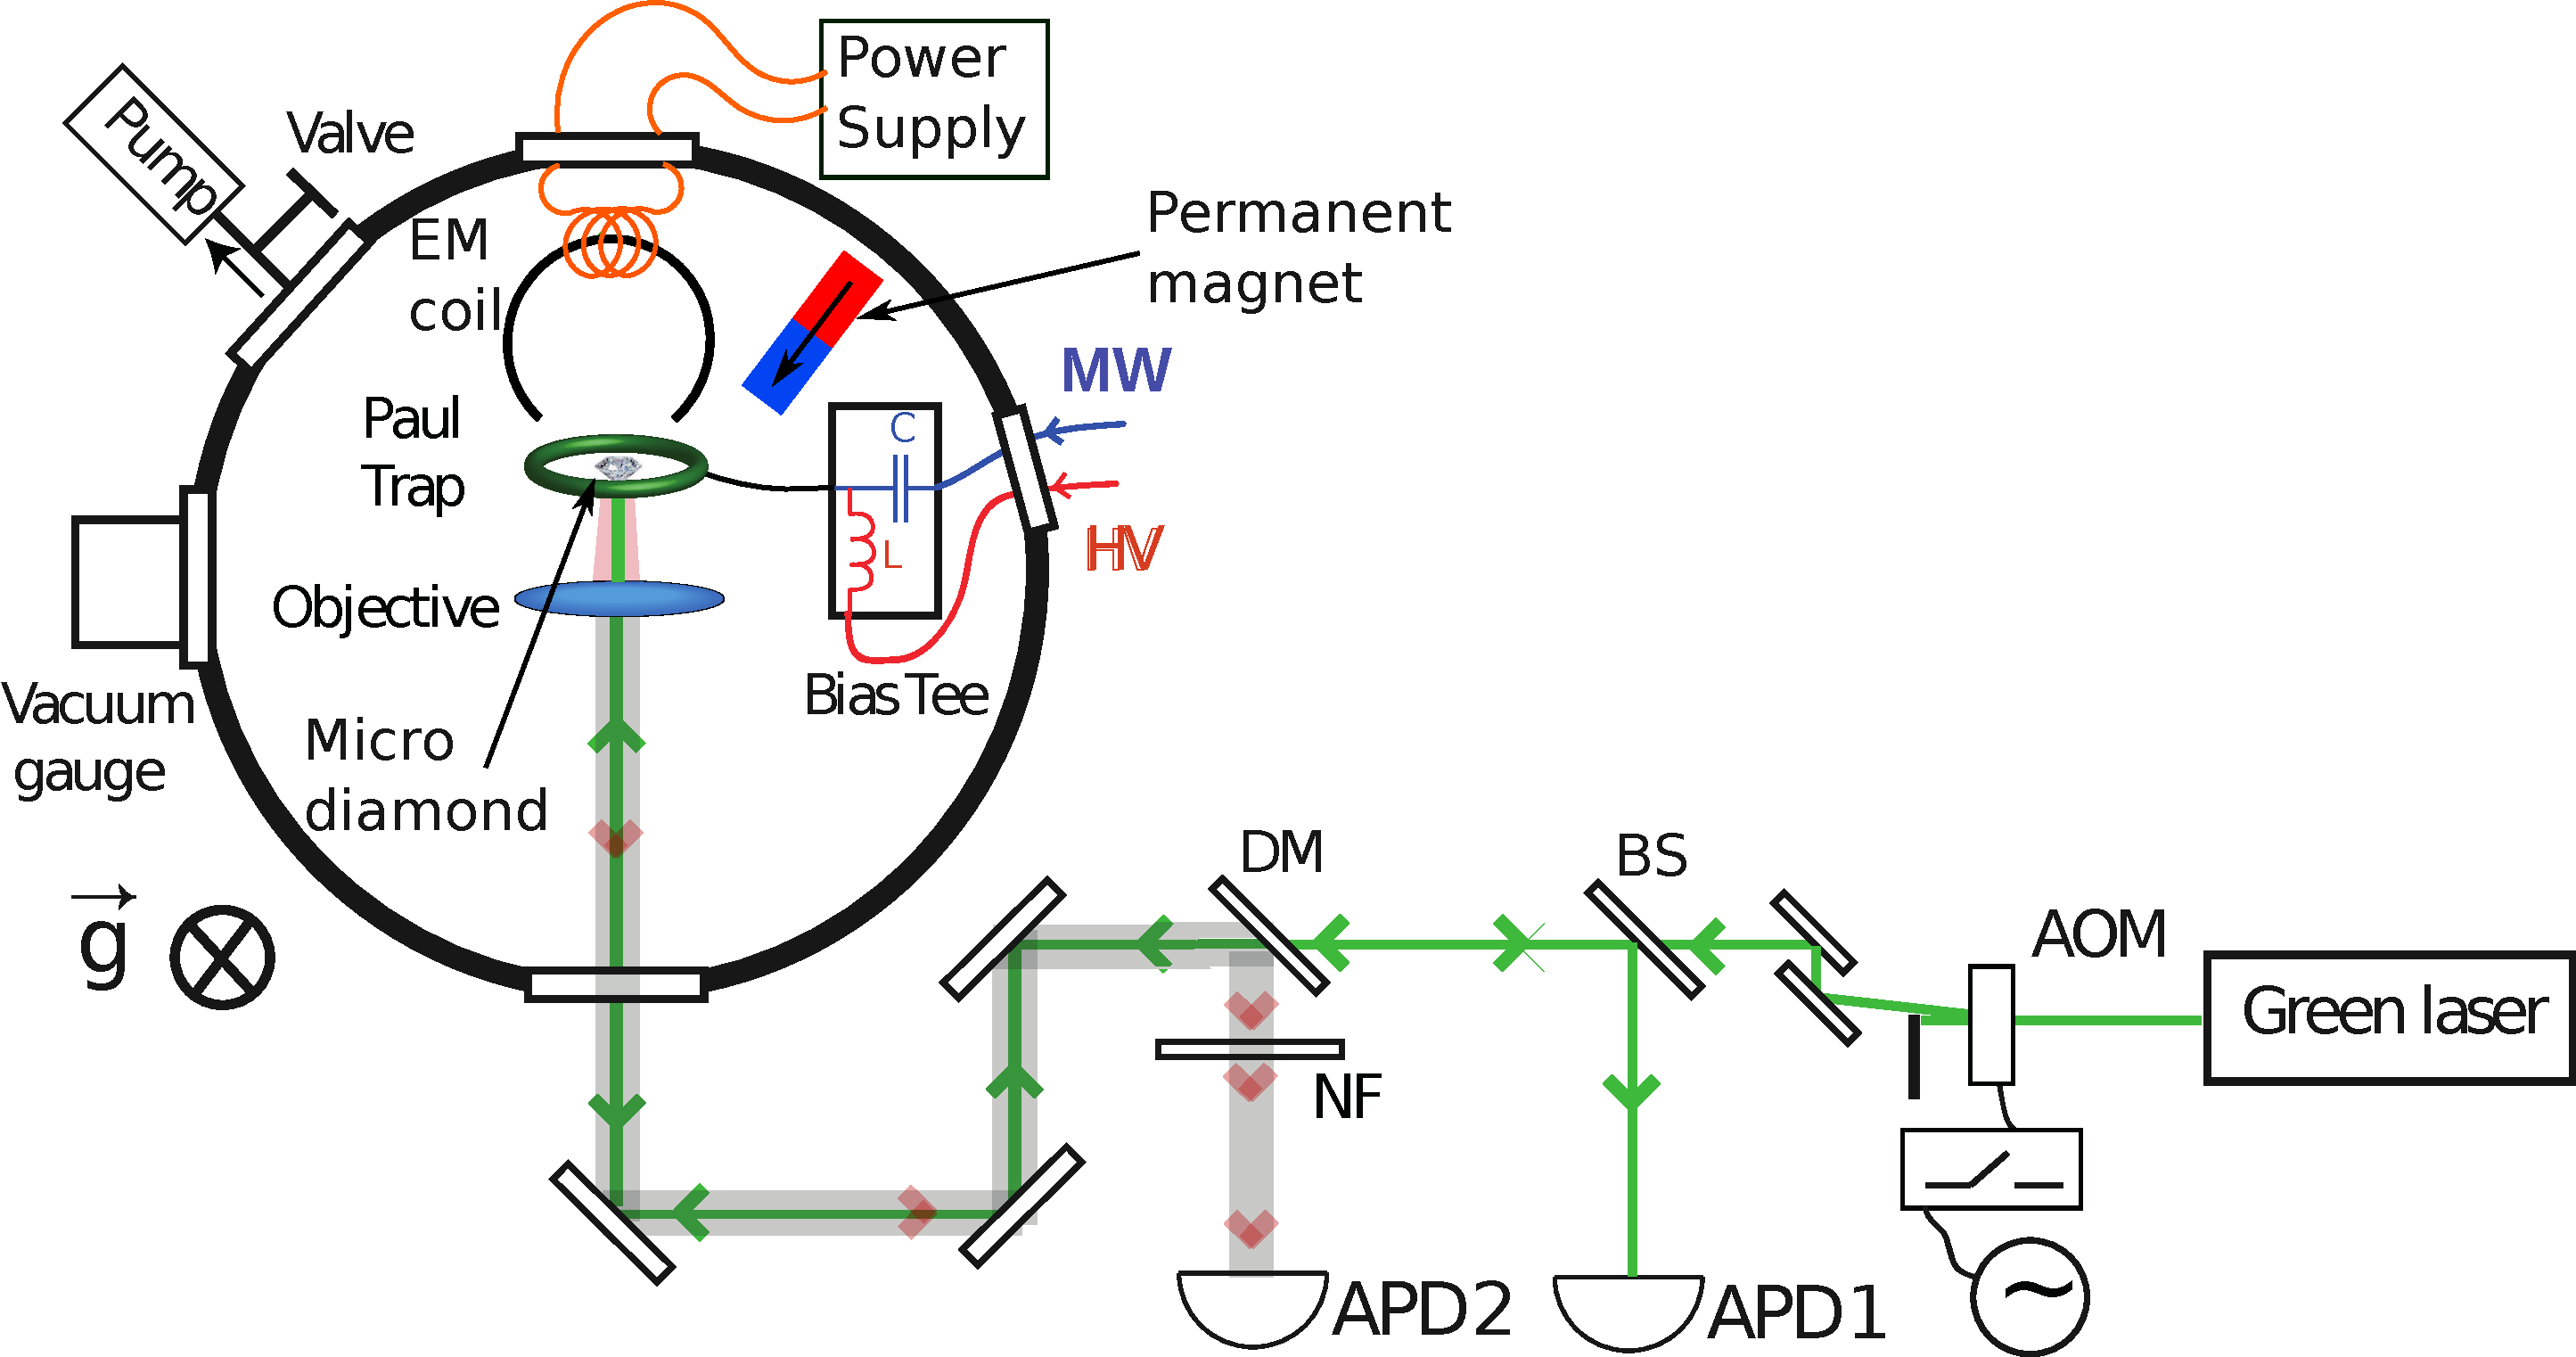
\includegraphics{setup}}
  \caption{Illustration of the experimental setup.}
	\label{Optics}
\end{figure}

The experimental setup illustrated in Fig.\ref{Optics} is similar to the one used in \citep{DelordPRL} with the addition of a permanent magnet and an electromagnetic (EM) coil in order to perform magnetic field scans. The diamond sample is typically illuminated with 1mW of 532 nm laser light, focused by an objective with a numerical aperture of 0.5. An acousto-optic modulator (AOM) is used to switch on and off the 532nm laser and to finely tuned its power. The photo-luminescence (PL) is collected by the objective, separated form the excitation light using a dichroic mirror (DM) and a 532nm notch filter (NF), and detected using a multimode-fiber single-photon avalanche photo-detector (APD) (SPCM-AQRH-15 from Perkin Elmer). Typically, from the heavily doped samples that we use, we can detect PL photons at a rate of 1 MHz after attenuating the signal by a factor 100 with neutral density filters. 
The Paul trap is a pseudo-ring with a diameter of approximately 200 $\mu$m, as can be seen in \citep{DelordPhD}. It acts both as trap through the high voltage (HV) and as a microwave (MW) antenna.

The magnetic field generated by the (homemade) EM coil is controlled by a programmable power supply (Rhode \& Shwartz NGE 103) performing current ramps.
While the levitating setup is located in a vacuum chamber, all the experiments presented in this article are performed at atmospheric pressure.

\subsection{$T_1$ measurement}
\begin{figure}[!ht]
  \centering \scalebox{1.2}{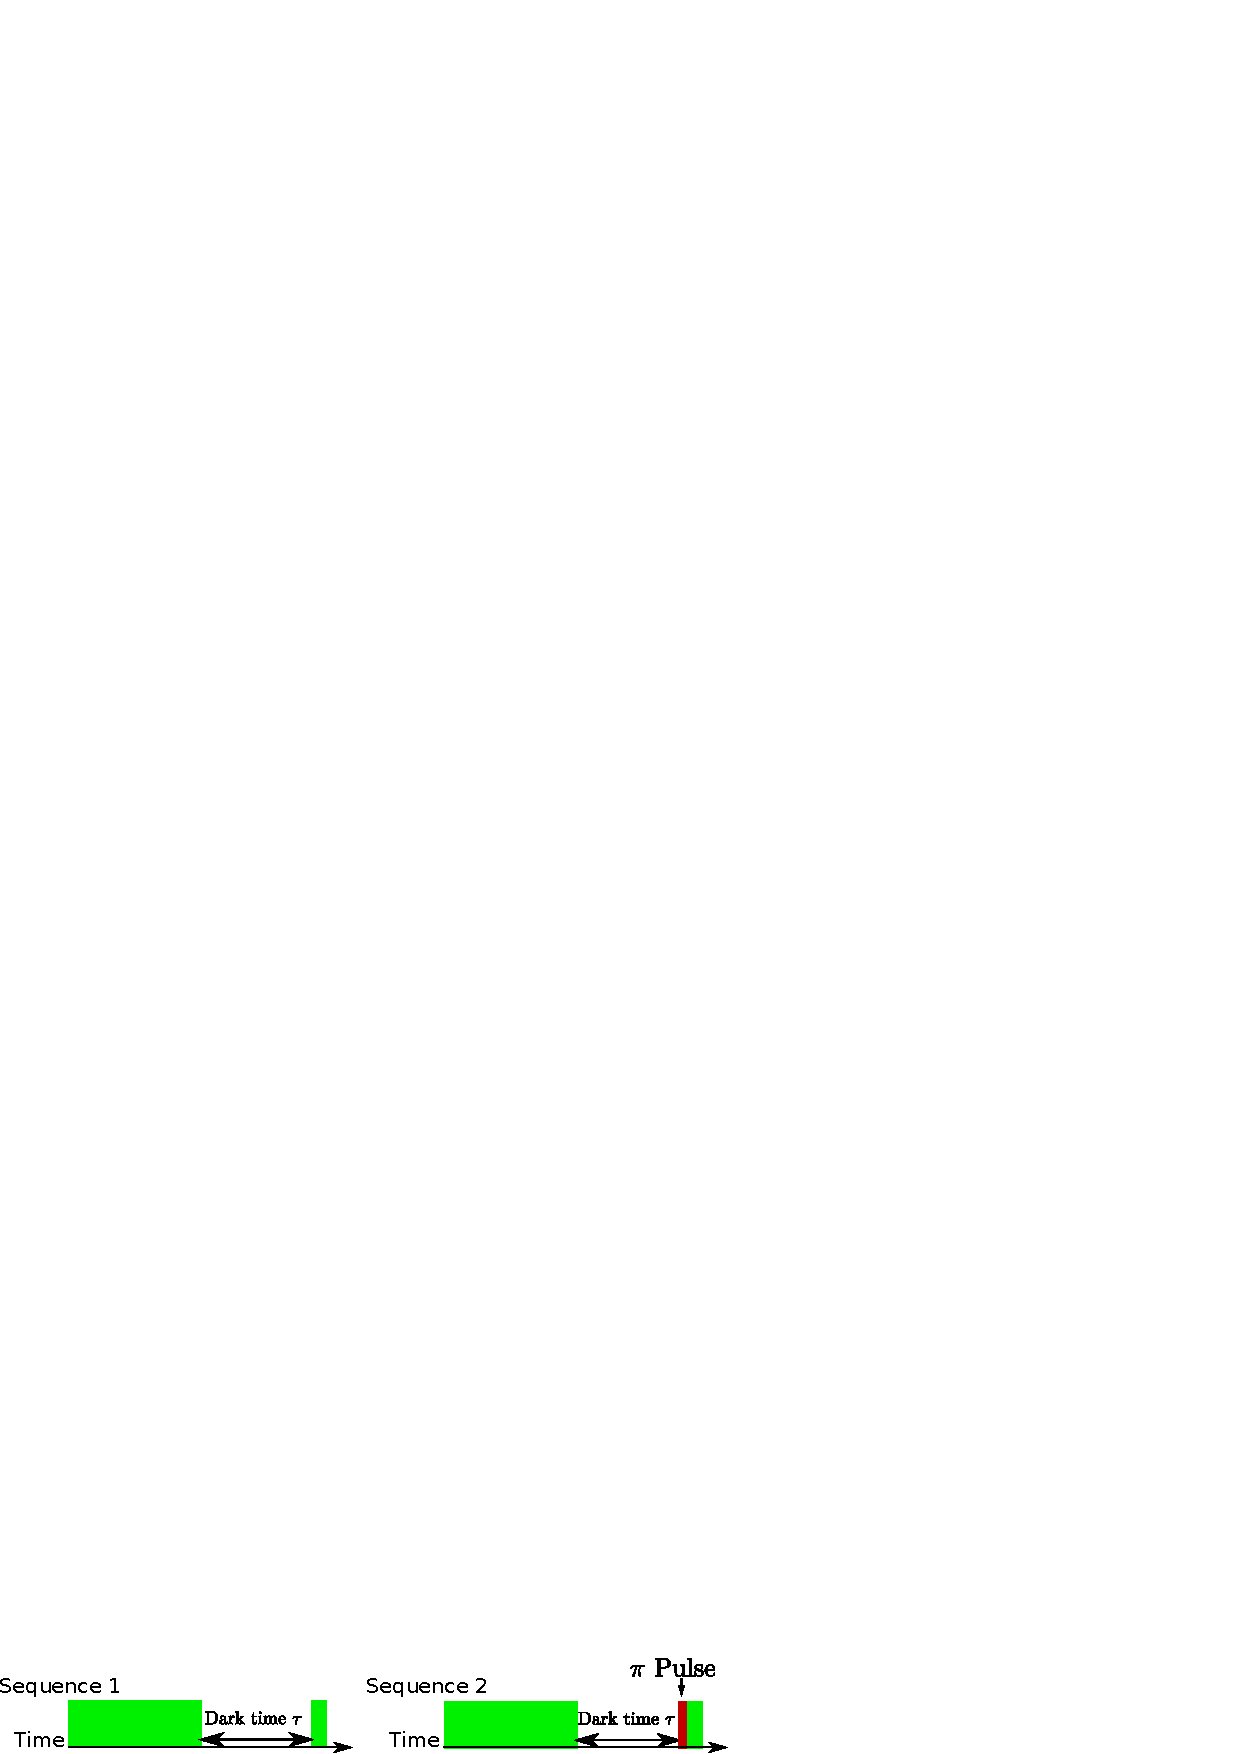
\includegraphics{T1_soustraction_shema}}
  \caption{$T_1$ measurement protocol. Green bars represent laser excitation, red bar represent resonant microwave $\pi$ pulse.}
	\label{T1_protocol}
\end{figure}

As shown in the Fig. 2-c) of the main text, the spin lifetime of the NV centers is modified in the presence of cross-relaxation with other classes of NV centers.
Here we present the protocol for removing the effects of charge state transfer in the dark, which mask the PL signal decay induced solely by spin depolarization. 
The protocol described in Fig. \ref{T1_protocol} consists in using two sequences. In the first sequence the spins are initially polarized in the $\ket{m_s=0}$ state through a 1 ms green laser excitation pulse and then left to evolve in the dark for a variable dark time $\tau$. The spin state is finally read out using a 10 $\mu$s laser pulse (shorter than the polarization time of the spins).

The second sequence uses the same parameters (polarization time, dark time and readout time) than the first sequence, but uses an extra resonant microwave $\pi$ pulse tuned to a transition of one of the four classes of NV$^-$ right before the readout pulse. The latter sequence brings population from the $\ket{m_s=0}$ state to the $\ket{m_s=\pm 1}$ state for one class of NV centers.

By measuring the difference between the two signals obtained in these two measurements, we can extract the evolution of the spin state population from a single NV class and, at the same time, remove unwanted contributions to the photoluminescence, such as charge state transfer in the dark (which give the same background contribution to the to the measurements).
In order to avoid low frequency noises such as laser drifts from the focal point or intensity fluctuations, we alternate both sequences while performing the measurement.

\subsection{Magnetic field calibration}

A neodymium permanent magnet and an electro-magnet are placed a few centimeters away from the diamond sample in order to apply a uniform and controllable magnetic field to the NV centers. 

To calibrate the magnetic field magnitude $B$, and its orientation $\theta$ with respect to the NV axis, we record Optically Detected Magnetic Resonance (ODMR) spectra and record two the frequency of two transitions $|0 \rangle \rightarrow |-1\rangle$ and $|0 \rangle \rightarrow |+1\rangle$ from the same class to determine both the angle of the B field with respect to this class and the magnetic field amplitude. 

\subsection{Spin-mechanical detection}

High sensitivity of the spin-torque is achieved by using a speckle pattern produced by the rough surface of the micro-diamond under coherent illumination. When the particle is stably levitating, at the particle image plane, we then focus a small area of the speckle image onto an optical fibre and detect the photons transmitted through the fibre with the APD$_1$. The detected signal is then highly sensitive to the particle position and orientation.

For the spin-torque measurements presented in Fig. 4-a), the microwave detuning is scanned in 2~MHz steps with a duration of 10 ms per points. During those 10ms, the diamond orientation has enough time to reach its equilibrium position and the spin torque effect can be observed. The average count-rate is about 1 Mega-counts/s. 

\subsection{Angular signal drift for levitating particles}

Measurements on levitating diamonds have to be relatively short (few minutes at most) because of a slow drift on the particle orientation which changes the detection location on the specular reflection off the diamond surface. The most likely origin of this drift is the loss of charges of the diamond due to photoionization by the laser, which changes the trapping conditions over time.

%This drift is the reason why the photoluminescence scan in Fig.3 of the main text has a lower signal to noise ratio than the scan in Fig.1 of the main text, which was done on a static diamond for a few hours.


%\subsection{PL detection}
%
%In these measurements, compared to \cite{DelordNat}, to detect the PL we use another detection channel that is more resilient to motion. We therefore do not need to detect prior to ring down.

\section{Principle of the mechanical detection}


\subsection{Origin of the magnetic torque}

The magnetic torque responsible for the motion of the diamond fundamentally comes from the anisotropy of the NV centers and from the transverse field $B_\perp$ responsible for mixing the eigenstates in the stationary state. We will start by considering the torque from a single NV center.
%The hamiltonian of a single NV under a magnetic field is 
%\be
%\hat{H}=\hbar D S_z^2+\hbar \gamma_e\bm S \cdot \bm B
%\ee
Without lack of generality, we will assume that the B field points in the $z$ direction and take the motion to be in the $x-z$ plane (in the lab frame), see Fig.~\ref{axes}.

\begin{figure}[ht]
\centering{ \scalebox{0.4} {\includegraphics{axes.eps}}}
  \caption{Notations used to define the axes in the body fixed and laboratory frames of reference $\mathcal{R'}$ and $\mathcal{R}$ respectively.}
  		\label{axes}
\end{figure}

In the body fixed frame, the magnetic part of the hamiltonian reads 
$\hat {H}_{B}= \hbar \gamma_e B  (\hat{S}_{x'} \sin\theta + \hat{S}_{z'} \cos\theta)$
where $\theta$ is the angle between the B field and NV center quantization axis $z'$.
We thus obtain the spin torque operator
\be
\hat \tau_s = -\frac{\partial \hat{H}}{\partial \theta} = \hbar \gamma_e B (-\cos\theta \hat{S}_{x'}+\sin\theta \hat{S}_{z'}).
\ee
The mean value of the torque operator in terms of the reduced density matrix elements $\rho_{ij}$ in the basis of the $S_{z'}$ eigenstates $|-1\rangle_{z'},|0\rangle_{z'},|1\rangle_{z'}$ is 
\be
\langle \hat \tau_s \rangle =\mathrm{Tr}_\mathcal{B}(\hat \rho \hat \tau_s) = \hbar \gamma_e B   (\rho_{-1-1}-\rho_{11})\sin\theta - \hbar \frac{\gamma_e B}{\sqrt{2}} S \cos\theta\label{torquemean}
\ee
where we introduced $S=\rho_{0,1}+\rho_{1,0}+\rho_{0,-1}+\rho_{-1,0}$.
The bath $\mathcal{B}$ over which the trace is performed consists of laser photons used to polarized the NV at a rate $\gamma_{\rm las}$, phonons or spin-fluctuators acting on the spin populations at a rate $\Gamma_1=1/T_1$ and 
$P_1$ centers or nuclear spins dephazing the electronic spin at a rate $1/T_2^*$.
In the limit $\gamma_e B \ll D$, and $\gamma_{\rm las}\gg \Gamma_1$ the laser efficiently polarizes the electronic spins in the ground state so that $\rho_{00}\gg {\rho_{11},\rho_{-1-1}}$.
The pure dephazing $T_2^*\approx 100$ns is much shorter than the sum of the population relaxation time $T_1/2 \le 1$ms and the laser induced repolarization time $1/\gamma_{\rm las} \le $ 100 $\mu$s. The equations of motion for the coherences thus read 

\bea
\frac{\partial \rho_{01}}{\partial t}&=&-\frac{1}{2T_2^*} \rho_{01}-i\frac{ \gamma_e B}{\sqrt{2}}\sin\theta-i\rho_{01}D+\mathcal{O}(\frac{(\gamma_e B)^2}{D})\\
\frac{\partial \rho_{0-1}}{\partial t}&=&-\frac{1}{2T_2^*}  \rho_{0-1}-i\frac{ \gamma_e B}{\sqrt{2}}\sin\theta-i\rho_{0-1}D+\mathcal{O}(\frac{(\gamma_e B)^2}{D}).
\eea
%Taking the complex value of these equations give the two other eq coherence terms. 
%The coherences can have an impact on the angle since they are responsible for the mean torque applied to the particle. 
The characteristic motional dynamics is very slow compared to the zero-field and magnetic field rates $D$ and $\gamma B$. The latter are also much larger then the decoherence rate $1/T_2^*$ in our experiments, so we can adiabatically eliminate the coherences and find 
\bea
\rho_{01}=\rho_{10}\approx-\frac{\gamma_e B \sin\theta}{\sqrt{2} D} \quad {\rm and} \quad \rho_{0-1}=\rho_{-10}\approx-\frac{\gamma_e B \sin\theta}{\sqrt{2} D}.\eea
Since 
\bea
\rho_{11}-\rho_{-1-1}=\mathcal{O}(\frac{\gamma_e B}{D}).
\eea 
Re-injecting these expressions in the expression for the mean torque, we get 
\bea
\langle \hat \tau_s \rangle = \frac{\hbar(\gamma_e B)^2}{D}\sin2\theta
 +  \mathcal{O}(\frac{(\gamma_e B)^3}{D^2}).\label{torque_anal}
\eea

It is in fact the gradient of the energy in the ground state taken at the angle $\theta$. 

Indeed, supposing that $\gamma B \ll D$, so that $H_{B}$ can be treated as a perturbation to the spin-spin hamiltonian $D \hat S_{z'}^2$, 
the perturbed energy $\epsilon_0$ of $\ket{0}$ is 
\bea \epsilon_g=\sum_{m_s=\pm 1}\frac{ |\bra{0} H_B \ket{\pm 1}|^2}{-\epsilon^0_{\pm 1}}=-\hbar\frac{(\gamma_e B)^2 }{D} \sin^2\theta
\eea

Taking $ -\partial \epsilon_g /\partial \theta$ then gives Eq. \ref{torque_anal}. It is the equation that is used in the core of the manuscript. 
In the approximate regime of the present study, the Hellmann-Feynman theorem (exact for pure states) that relates the angular derivative of the mean energy to the torque is correct in the above-described limits where dissipation is negligible. \\

\begin{figure}[ht]
\centering{ \scalebox{0.4} {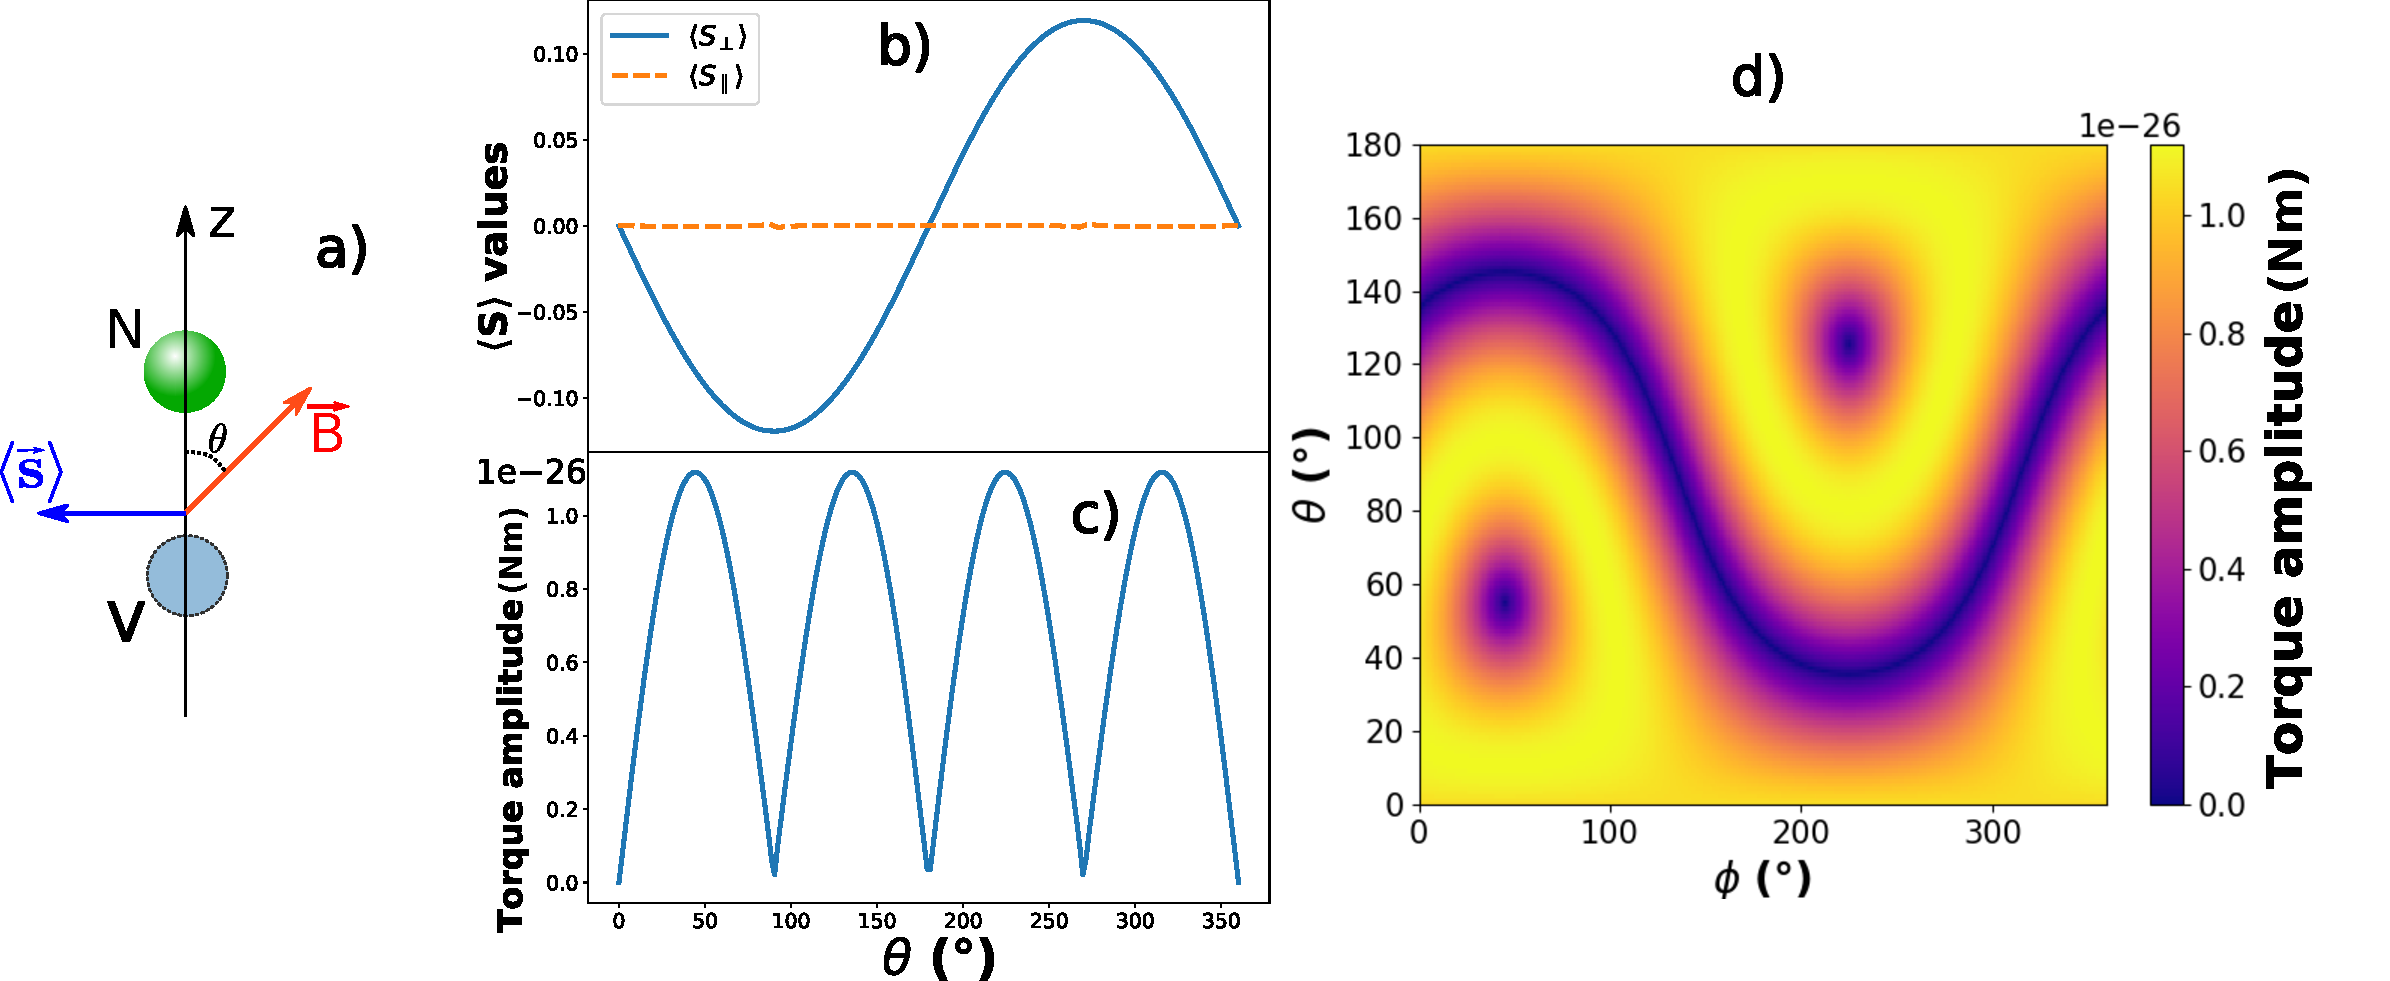
\includegraphics{map_torque_1_classe}}}
  \caption{\textbf{a)} Skecth showing an NV center aligned to the \textbf{z'} direction in the presence of an external magnetic field \textbf{B} at an angle $\theta$ with respect the NV axis. The resulting spin vector $\langle \mathbf{ \hat S} \rangle$ of the NV center is shown by the blue arrow.
   \textbf{b)} Longitudinal ($S_\parallel$ in dashed line) and transverse ($S_\perp$ in plain line) components of the average value of the spin operator, in $\hbar$ unit, as a function of $\theta$ and for a magnetic field amplitude $|\mathbf{B}|=100$ G.   
   \textbf{c)} Amplitude of the magnetic torque acting on a single spin as a function of $\theta$ for $|\mathbf{B}|=100$ G.
   \textbf{d)} Amplitude of the same magnetic torque in the crystalline basis with $\theta$ and $\phi$ being the polar and azimuthal angle with respect to the [100] direction.}
  		\label{Torque1classe}
\end{figure}


Another way to estimate the torque is to numerically solve the master equation of the system as depicted in Fig \ref{Torque1classe}. We find that under green excitation and in the presence of an external magnetic field, the spins will acquire a magnetization $\gamma_e \langle\hat{\mathbf S}\rangle$ which, under the low magnetic fields ($<$ 200 G) we are working at, will be oriented at an angle of 90$^\circ$ from the NV axis : $\langle \hat S_{z'} \rangle \approx 0$ and $\langle \hat S_\perp \rangle \neq 0$. This magnetization vanishes when the magnetic field is aligned with the NV center since there is no longer a transverse field responsible for the mixing of the eigenstates. 

The magnetization of the NV center is therefore not aligned with the magnetic field, except when the field is also at a 90$^\circ$ angle from the NV axis, which means that the magnetic torque $\mathbf \Gamma = \gamma_e \langle\hat{\mathbf S}\rangle \times \mathbf B $ will be non-zero everywhere except when the field is aligned with the center, or in the plane normal to the direction of the center. We can describe each NV center as a paramagnetic defect with the anisotropic magnetic susceptibility $\chi = \begin{pmatrix}-\chi_\perp & 0 & 0\\ 0 & -\chi_\perp & 0 \\ 0 & 0 & 0  \end{pmatrix}$ in the $(\mathbf{x'},\mathbf{y'},\mathbf{z'})$ basis where $\mathbf{z'}$ is the orientation of the NV center.

The amplitude of the torque with respect to the magnetic field orientation at a B field amplitude of 100 G is represented in 1D in Fig \ref{Torque1classe}-c) where we can see a behavior very close to $|\sin(2\theta)|$, as found in Eq.\ref{torque_anal} through a perturbative approach. The same torque amplitude is represented in 2D in Fig \ref{Torque1classe} d). The two purple dots in the map correspond to the [111] direction when the magnetic field is aligned with the centers. The curvy line corresponds to the (111) plane. Importantly, the maximum torque value is $1\cdot 10^{-26}$ N.m for a single spin.

\subsection{Total spin torque and influence of cross-relaxation}

%\begin{figure}[ht]
%\centering{ \scalebox{0.4} {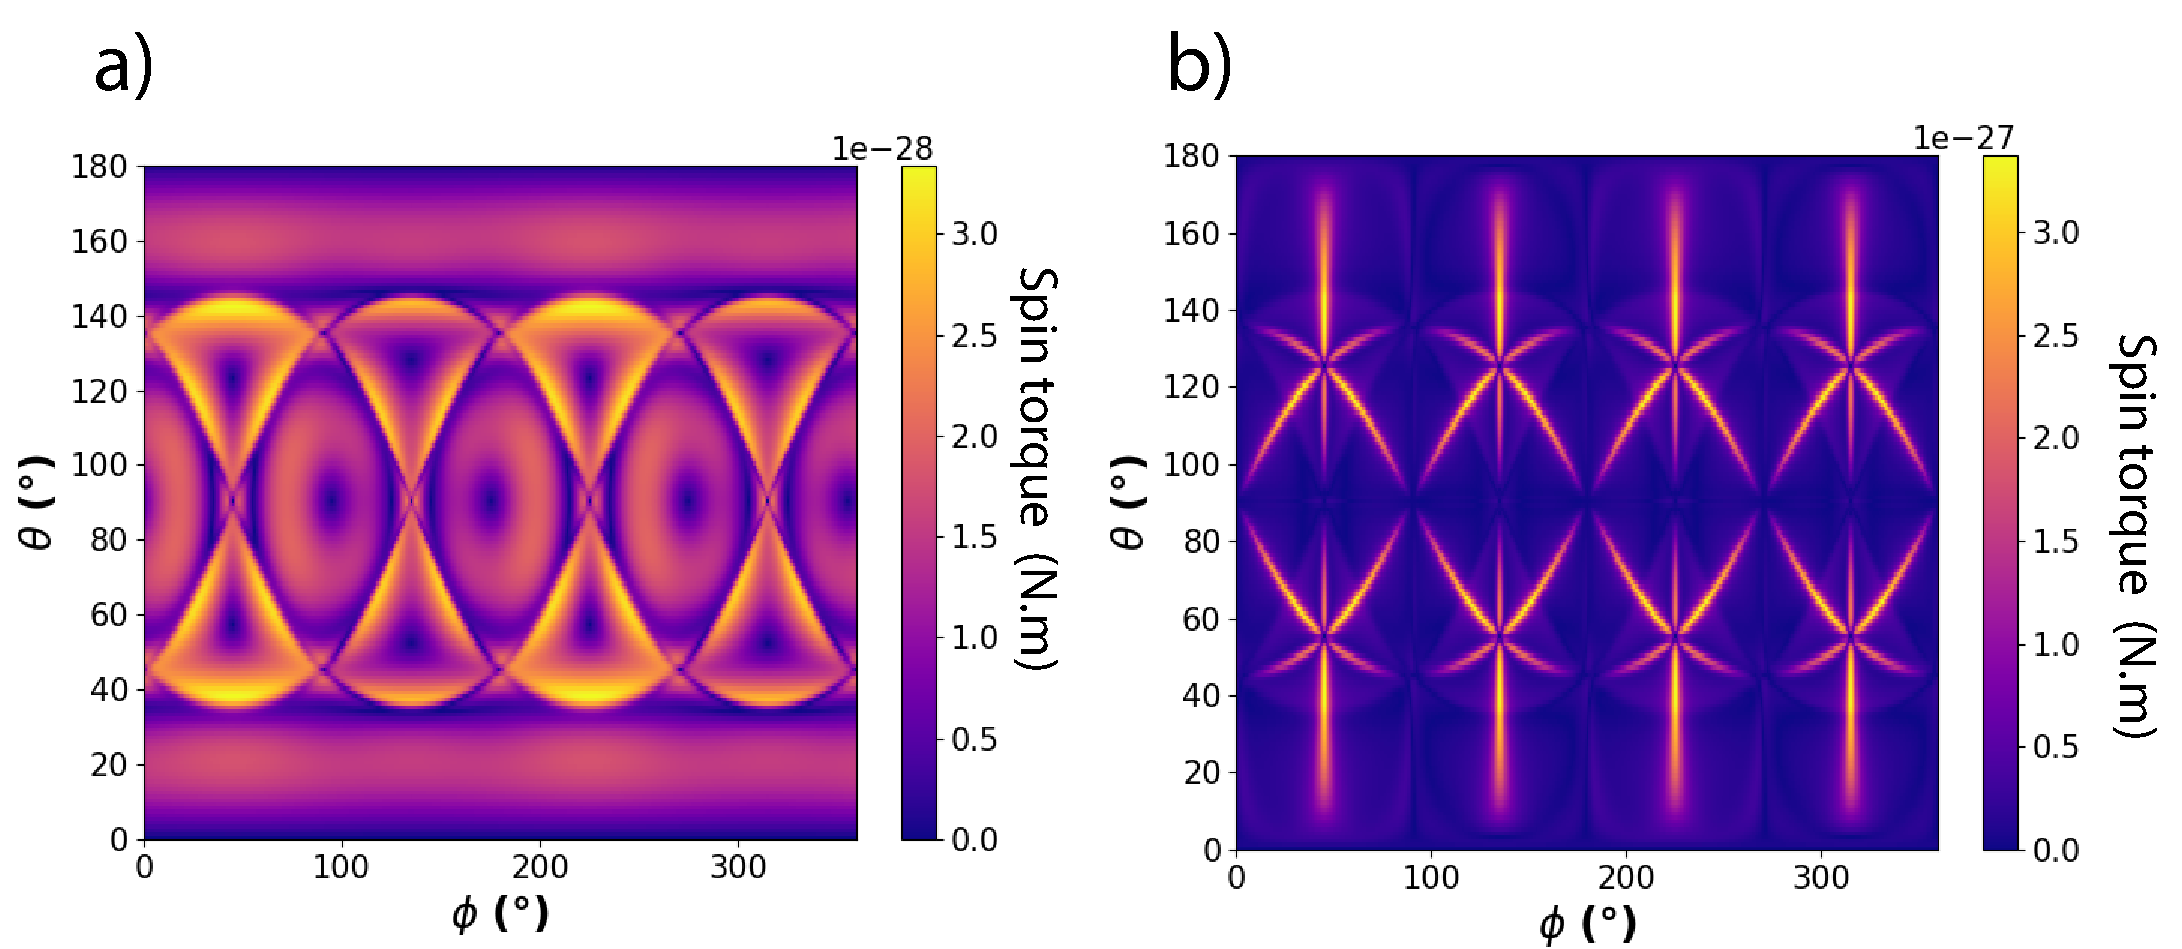
\includegraphics{map_torque_4_classe}}}
%  \caption{Magnetic torque amplitude for 4 spins, one in each possible orientation, as a function of $\theta$ and $\phi$, the polar and azimuthal angle with respect to the [100] direction. \textbf{a)} Not taking into account the CR between NV centers. \textbf{b)} Taking into account the CR between NV centers.}
%  		\label{Torque4classes}
%\end{figure}

Fig 3 a) in the main text, represents the same map as Fig \ref{Torque1classe}-c) but including the four NV centers, one in each of the possible [111] orientations. We can see that the maximum torque actually decreased to $3\cdot 10^{-28}$ N.m even though we increased the number of NV centers by four. This is due to the directional averaging of the torque generated by the four centers. The torque per NV center is decreased by more than two orders of magnitude when taking the directional averaging into consideration.
Fig 3 b) in the main text shows the same map, this time taking into account the modification of the spin lifetime due to cross-relaxations. The detailed model is presented in the section \ref{Simu}.
There are two things to note here : 
\begin{enumerate}
\item The maximum torque has increased by an order of magnitude compared to the previous case. It reached up to $3\cdot 10^{-27}$ N.m for four spins, so about $10^{-27}$ Nm per spin. Qualitatively, this is because cross-relaxation will lower the torque contribution of specific classes (the ones that get depolarized), meaning that the end result is closer to the single spin case (there is less directional averaging).
\item The change in magnetic torque is resonant, it happens only when different classes are brought to resonance. This can be seen by comparing Fig 3 b) of the main text to the $\{ 110 \}$ planes that were drawn in Fig. \ref{cristallo}. The change in the signal when scanning a magnetic field across a CR will be much sharper than the sinusoidal change in the spin-torque.
\end{enumerate} 

\subsection{Torque sensing with a levitating diamond}

The way we experimentally measure spin-torques applied on the levitating diamond is by measuring the induced diamond orientational displacement from equilibrium. 
We model the trap as a pure harmonic potential, both for the center of mass and for the librational degrees of freedom of the diamond with trapping frequencies $\omega_t \approx (2\pi) \cdot 1$ kHz. Considering a single librational degree of freedom, we can write the torque exerted by the trap as $\Gamma_t=-K(\theta-\theta_{eq})$, where $K=I \omega_t^2$ is the stiffness of the trap, $I$ being the moment of inertia of the diamond.

The application of an external torque $\Gamma_{\mathrm{ext}}$ to the diamond will therefore shift the angular equilibrium position  in such a way that : 
\begin{align}
-K(\theta-\theta_{\mathrm{eq}}) + \Gamma_{\mathrm{ext}} &= -K(\theta-\theta_{\mathrm{eq}}') 
\end{align}
so that
\begin{align}
\delta\theta = \theta_{\mathrm{eq}}'-\theta_{\mathrm{eq}} &= \frac{\Gamma_{\mathrm{ext}}}{K}=\frac{\Gamma_{\mathrm{ext}}}{I \omega_t^2}
\end{align}

In our case, $\Gamma_{\mathrm{ext}}$ is the magnetic torque exerted by the NV$^-$ spins on the diamond. We can write it $\Gamma_{\mathrm{ext}} = N_{NV} \langle \Gamma_{\mathrm{1 spin}} \rangle$  where $\langle \Gamma_{\mathrm{1 spin}} \rangle = \gamma_e \langle\hat{\mathbf S}\rangle \times \mathbf B \approx 10^{-27}$ Nm is the expected magnetic torque applied by one spin.

By using the inertia moment formula of a sphere : $I=\frac{2}{5}m r^2$, we can then rewrite the angular displacement as $$ \delta\theta = \frac{\langle\Gamma_{\mathrm{1 spin}}\rangle n(NV^-)}{\frac{2}{5}m_Cr^2\omega_T^2} \approx 10^{-3} rad$$ where $n(NV^-) \approx 5 \cdot 10^{-6}$ (5 ppm) is the number of NV centers per atoms in the crystal, $m_C \approx 2 \cdot 10^{-26}$ kg is the average weight of a carbon atom (we assume that the bulk of the diamond weight comes from carbon atoms), $r= 7.5$ $\mu$m is the typical radius of our diamonds and $\omega_T = 6.3\cdot 10^3$ rad/s is the typical value of the trap angular frequency.

It should be noted that the main uncertainty comes here from the diamond size which can change the expected result by an order of magnitude.

\section{Cross-relaxation detection for another type of degeneracy}

%Faire 2 lignes avec sur la première ligne l'ESR et le trajet sur la carte du champ mag
\begin{figure}[!ht]
  \centering \scalebox{0.4}{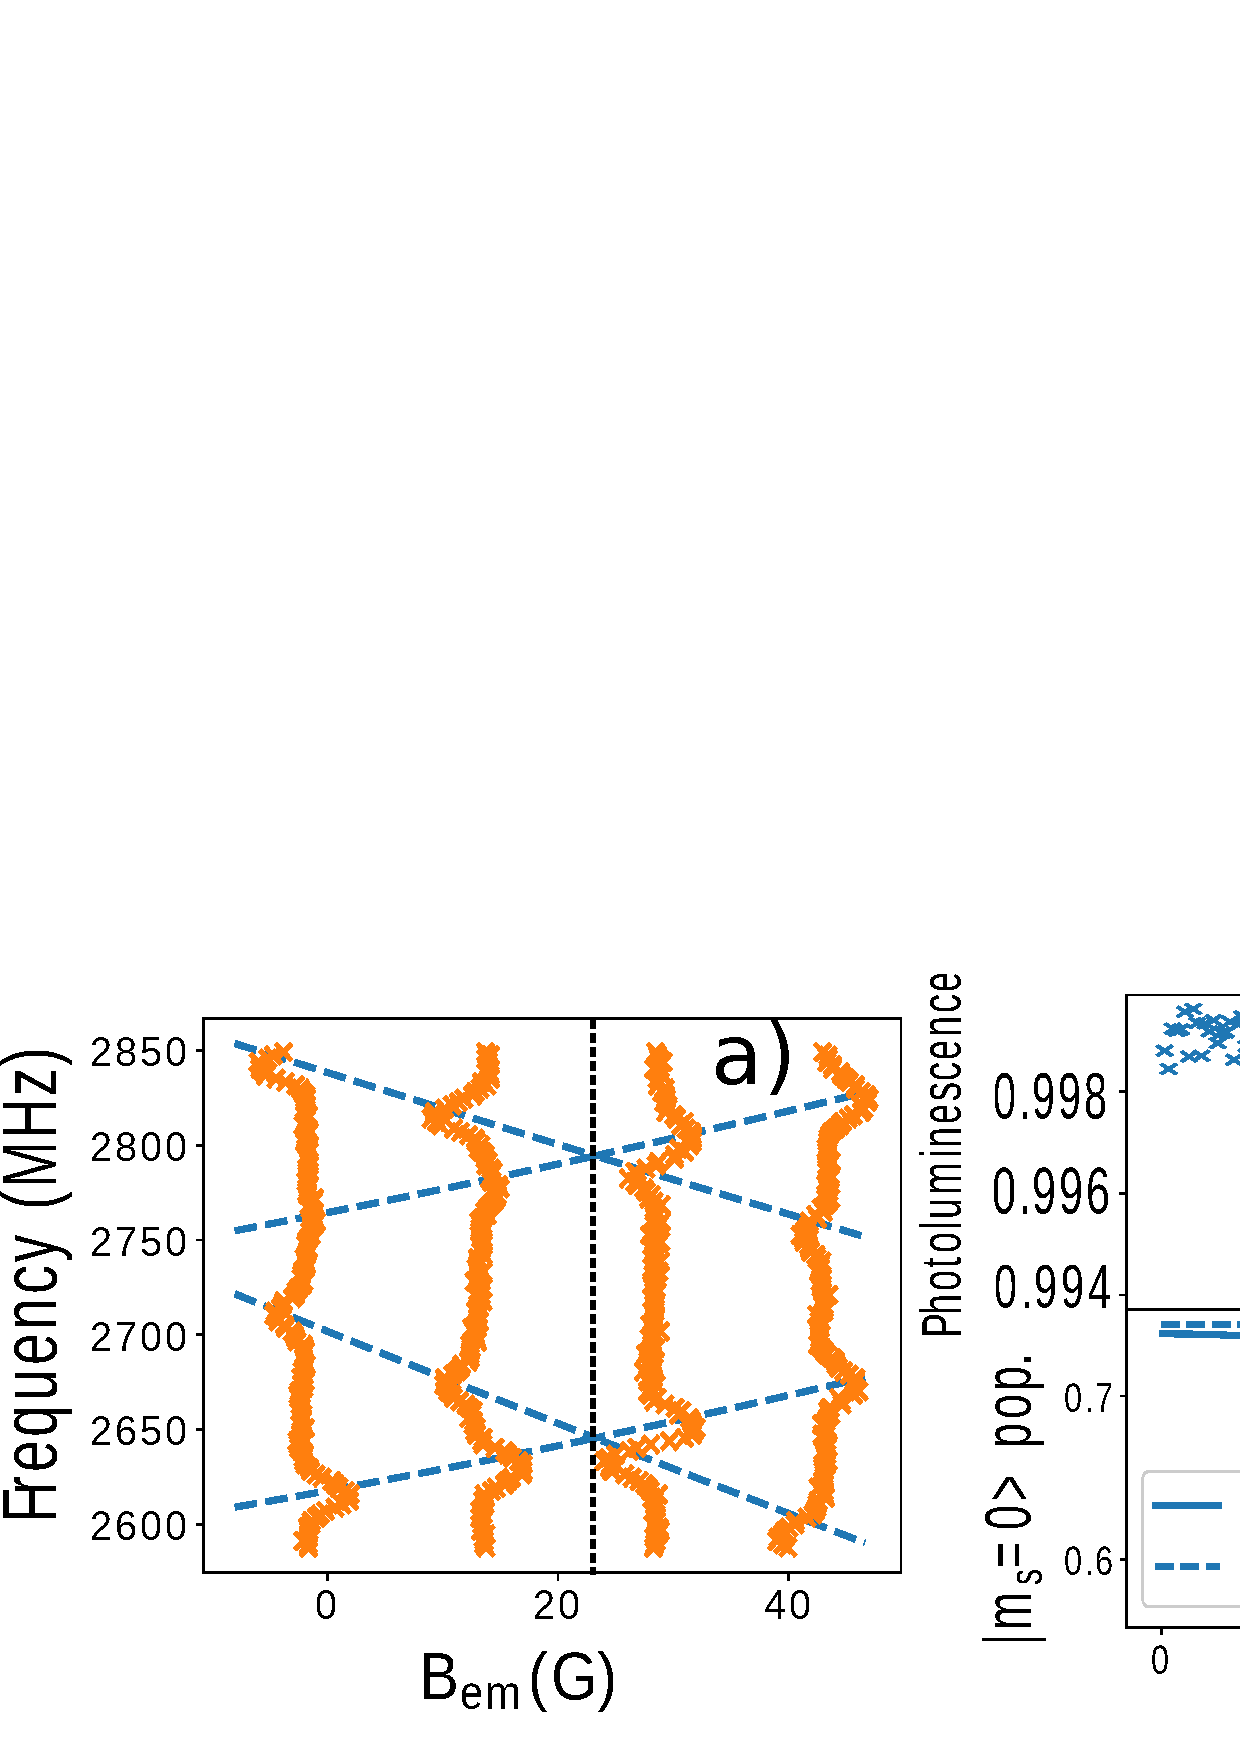
\includegraphics{22-total}}
  \caption{Mechanical detection of a dipolar interaction wen crossing a [100]$_\perp$ plane. \textbf{a)} Path of the magnetic field angle (red dots) in the ($\theta , \phi$) basis in the measurements, with respect to the [100] direction. The [100]$_\perp$ family of planes are shown in plain blue lines. The [110]$_\perp$ family of planes is shown in orange dashed lines. \textbf{b)} ESR spectra measured at 4 different magnetic field values. Calculated evolution of the NV transition frequencies as a function of the electromagnet B field $B_{\rm EM}$, for the four $\ket{0} \to \ket{-1}$ transitions (dashed lines). \textbf{c)} Photoluminescence of the NV centers as a function of the scanning magnetic field (blue crosses) and gaussian fit (orange line). \textbf{d)} Simulated population in $\ket{m_s=0}$ for the stationary state with (plain) or without (dashed) taking into account the decrease of the T$_1$ induced by the cross-relaxations.
  \textbf{e)} Signal reflected off the diamond surface as a function of magnetic field amplitude $B_{\rm EM}$ (blue crosses). The orange line shows a double gaussian fit. \textbf{f)} Simulated torque applied by the spins on the diamond, with (plain) or without(dashed) taking into account the cross-relaxations.}
	\label{CR_22}
\end{figure}

Similarly to in Fig. 3 of the main text, we managed to mechanically detect other types of mechanically induced dipolar couplings.
Fig. \ref{CR_22}b) shows a calculation of the frequencies of the $\ket{0} \to \ket{-1}$ transitions for all four classes of NV centers and the mechanically detected ESR spectra measured using the reflected laser for various magnetic field values. Unlike the experiment reported in the main text, this time all four classes of NV are resonant with another class at B=23 G. This indicates that we are crossing a [100]$_\perp$ plane instead of a [110]$_\perp$ one, as can be seen in Fig \ref{CR_22}a).

Fig. \ref{CR_22}c) shows the recorded photoluminescence of the NV centers during the magnetic field scan. As expected, a drop in the photoluminescence rate is observed when the degeneracy occurs. The PL drop is slightly more pronounced in this case compared to the experiments presented in the main text because all classes are depolarized here, instead of only two. This is well predicted by the numerical estimates shown in Fig. \ref{CR_22}d).

Fig. \ref{CR_22}e) shows the signal of the laser reflected off the diamond surface, proportional to the angular displacement. Here, there is a clear difference between the angular response and the experiment shown in the main text. Instead of a single Gaussian drop centered on the CR resonance, two bumps are observed on both sides of the resonance. 
Fig. \ref{CR_22}f) shows the result of simulations, where we can see a dispersive profile with an almost zero torque at the resonance. 
The reason we do not observe a change of sign in the experiment (with two positive bumps instead of a positive and negative one) is likely to be because of the non-linearity of our detection : if the signal initially corresponds to a dark spot of the speckle, then a change in the motion of the diamond can only result in an increased signal. 

Let us give a physical interpretation of the dispersive angular profile for this degeneracy condition. 
Here, the magnetic torque generated by the four classes of NV is not modified exactly on resonance, since all four classes are depolarized identically. Close to resonance, all classes will not be identically depolarized however : looking at Fig. \ref{CR_22}b), we can see that the two classes which have a higher frequency are always slightly closer to each other than the two classes of lower frequency. This can be since by computing the slope in the evolution of the transitions frequencies, which are found to be smaller for the two upper classes. 
This effect results in more depolarization for these two classes, except when they are exactly on resonance. This interpretation explains the overall shape of the torque and thus of the angular response.
A quantitative analysis would require knowledge about the directions of the 4-NV directions with respect to the three main directions of the trapped diamond axes as well as a calibration of the sensitivity of the speckle detection method for the three corresponding angular modes. 

\section{Simulation details}
\label{Simu}
In this part we will discuss the method used to simulate the average torque as well as the population in the $\ket{m_s=0}$ state. Numerical solving of the master equation was performed using the Quantum Toolbox in Python (QuTiP) \citep{qutip1} \citep{qutip2}.

In order to describe the dynamics of our spin ensemble, we introduce a incoherent optical pumping through the jump operators $\mathcal{L}_+ = \Gamma_l \ket{0}\bra{+1} $ and $\mathcal{L}_- = \Gamma_l \ket{0}\bra{-1} $, where $\Gamma_l \approx (2\pi) 10$ kHz is the laser induced polarizing rate to the ground state.
We also introduce the usual $T_1$ jump operators $\mathcal{L}_i^j= \frac{1}{T_1}\ket{i}\bra{j}$ where $\ket{i,j}$=$\ket{0, \pm 1}$.

In order to describe the $T_1$ modification induced by the cross-relaxations, we use a phenomenological model where each class has its own T$_1^i$ ($i \in \{1,2,3,4\}$) that depends on the energy levels of the other classes with the formula :
\begin{equation*}
\frac{1}{T_1^i}=\frac{1}{T_1^0}+\sum_{j \neq i} \frac{1}{T_1^{dd}}e^{-\frac{(\nu_i-\nu_j)^2}{2(\sigma^{dd})^2}},
\end{equation*}
where $\nu_i$ and $\nu_j$ are the transition frequencies of the classes $i$ and $j$ (we are arbitrarily considering the $\ket{0} \to \ket{-1}$ transition here, since the resonance condition is the same for both transitions at the magnetic fields we are working at. This is not always true for magnetic fields greater than 592 G\citep{van_oort_cross-relaxation_1989}). 
$\sigma^{dd} $ is the width of the CR features. We measured them to be similar to the inhomogeneous broadening given by the dipolar coupling to $P_1$ centers, {\it i.e.} $\approx$ 6 MHz.  

$T_1^0=1.03$ ms and $T_1^{dd}=0.38$ ms were chosen to match the $T_1$ measurements presented in Fig. 1 of the main text. We only focus on the $T_1$ without degeneracy and the one with a single degeneracy since our experiments will not have more than two resonant classes at once. Our model is probably not suited to deal with triple our quadruple resonances.

Finally, according to previous measurements performed in \citep{choi_depolarization_2017}, only the $\ket{0}\bra{\pm1}$ and $\ket{\pm1}\bra{0}$ (corresponding to a single quantum exchange in the dipole-dipole interaction) operators are modified by the cross-relaxations. Using this model, we can numerically solve the master equation and get the density matrix in the stationary state $\rho_s$. With $\rho_s$ we can directly obtain the $\ket{m_s=0}$ population, corresponding to the experimentally measured photoluminescence.

With regards to the torque estimation, we use a semi-classical formula :
\begin{equation*}
\mathbf \Gamma = N_0 \gamma_e \langle\hat{\mathbf S}\rangle \times \mathbf B,
\end{equation*}
where $N_0 \approx 10^9$ is an estimate of the number of spins in our sample based on the average size and NV density of our diamonds, $\gamma_e$ is the gyromagnetic ratio of the electron and $\langle\hat{\mathbf S}\rangle =\mathrm{Tr}(\rho_s \mathbf{\hat S})$ is the averaged spin vector in the stationary sate, averaged again over the four possible orientations of NV.
This formula assumes that the spin dynamics is faster than the dynamics of the motion of the diamond, which is the case in our experiments.

In our plots in Fig. \ref{CR_22} and Fig. 3 of the main text, we only represent one spatial component (e.g. $\Gamma_x$) of the torque, because the three components behave similarly.
\bibliography{trap}

\end{document}
